\chapter{Einleitung}\label{chap:einleit}
\section{Projektbeschreibung}\label{sec:projektbeschreibung}

In den Schulen ist die Mensa manchmal gut und manchmal nicht so gut. Man kann
nie Wissen, wie gut das Essen ist, bis man es gekauft hat. Dieser
Problemstellung widmet sich dieses Projekt, welches das Essen an der Mensa der
Neuen Kantonsschule Aarau bewerten soll. Genauer soll das Essen von den
Schülern/Kunden selbst bewertet werden. So kann man, bevor man das Essen kauft
bereits einen Einblick in das Essen erhalten und sehen, wie gut es den Leuten
geschmeckt hat.

Das Projekt ist insofern spannend, weil viele Schüler gar nicht mehr die Mensa
besuchen. Das liegt daran, dass sie bereits schlechte Erfahrungen mit dem Essen
gemacht haben. Vielleicht lässt sich mit diesem Projekt die Mensa verbessern und
die Schüler wieder in die Mensa locken.

Es gibt bereits schon viele verschiedene Bewertungsportale für Restaurants und
andere Geschäfte. Dennoch sollte dieses Projekt etwas besonderes
zurechtgeschnittenes für allein die Mensa der Neuen Kantonsschule Aarau werden.
Aus diesem Grund ist diese Arbeit eine Engeneering Arbeit.

Um diese Arbeit umzusetzen braucht es Kenntnise in den Bereichen:
\begin{itemize}
    \item Datenbanken
    \item Webseiten Frontend
    \item Webseiten Backend
    \item Design
    \item Netzwerke
\end{itemize}

Die Arbeit nutzt für die Umsetzung folgende Technologien:
\begin{itemize}
    \item Libraries
    \subitem Django
    \subitem Requests
    \subitem BeautifulSoup
    \item Sprachen
    \subitem Python
    \subitem HTML
    \subitem CSS
    \subitem JavaScript
    \item IDE
    \subitem Visual Studio Code
\end{itemize}

\subsection{Architektur der Datenbank}
\begin{figure}[ht]
    \centering
    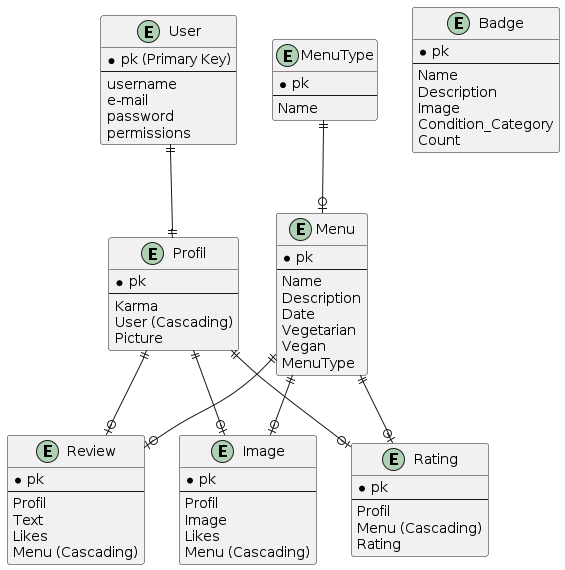
\includegraphics[width=0.8\textwidth]{images/Database.png}
    \caption{Architektur der Datenbank siehe auch \ref{code:models.py}}
    \label{fig:DB}
\end{figure}

\subsection{Architektur der Webseite}
\begin{figure}[ht]
    \centering
    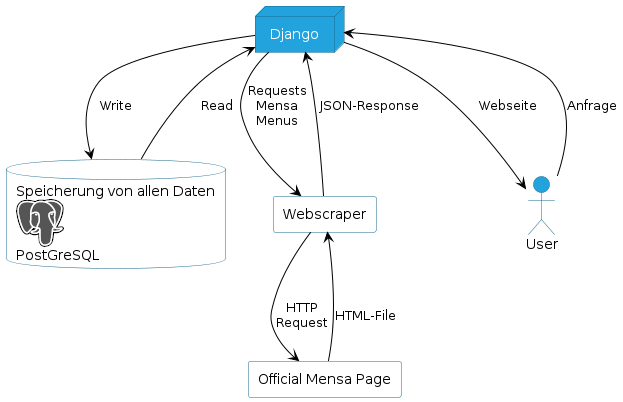
\includegraphics[width=0.8\textwidth]{images/Webseite.png}
    \caption{Architektur der Webseite}
    \label{fig:Website}
\end{figure}

\section{Problemdefinition}\label{sec:problemdefinition}
